\chapter{tentmaker Reference}
\label{chap:tentref}

This chapter explains how to start tentmaker, then gives a careful guided
tour of its tabs.

\section{Starting Tentmaker}

There are three ways to start tentmaker.  All of them allow an optional
port flag -p or --port, which allows you to change from the default port
of 8080.

\subsection*{Starting tentmaker in normal mode}

If you are happy with the table structure of your app, but you need to
work on some of its details, you can start tentmaker like this:

\begin{verbatim}
tentmaker file.bigtop
\end{verbatim}

You can even leave out the file, then tentmaker will start up with a default
file to get you started.  All of that is far too much work for the typical
Perl programmer, so read on.

\subsection*{Starting an app from scratch with tentmaker}

Use the -n or --new flag to start a brand new app in tentmaker.  This flag
expects an application name and a list of table relationships, like this:

\begin{verbatim}
tentmaker -n Sample table1 table2
\end{verbatim}

Keep in mind that tentmaker is not all that smart.  If you name one of
your tables with an SQL reserved word (table being the most popular) it won't
know or care or try to stop you.

\subsection*{Adding tables to an app with tentmaker}

If you already have a bigtop file, you may choose to augment it with
tentmaker.  While you could just start tentmaker in normal mode and do
all the work, you could also say something like:

\begin{verbatim}
tentmaker -a docs/sample.bigtop table3 table4
\end{verbatim}

\subsection*{Table relationships on the command line}

You can run both tentmaker and bigtop with the new and add mode
flags shown above.  In addition to merely adding tables, you can show
table relationships during this step.  For example, suppose I have a
new app which needs to track our hiring process.  For a start it will have
tables for job descriptions, job skills, and open positions.  I could
create the app like this:

\begin{verbatim}
tentmaker -n Hiring 'pos->job job<->skill'
\end{verbatim}

This will start the tentmaker.  If you wanted to build the app directly
and delay or completely avoid tentmaker, you could substitute bigtop
for tentmaker:

\begin{verbatim}
bigtop -n Hiring 'pos->job job<->skill'
\end{verbatim}

The details of table relationships were covered near the beginning
of Section \ref{sec:asciiart}.

\section{Tentmaker's Tabs}

Recall from Chapter \ref{chap:simpleex} that there are five tabs in
tentmaker:

\begin{figure}
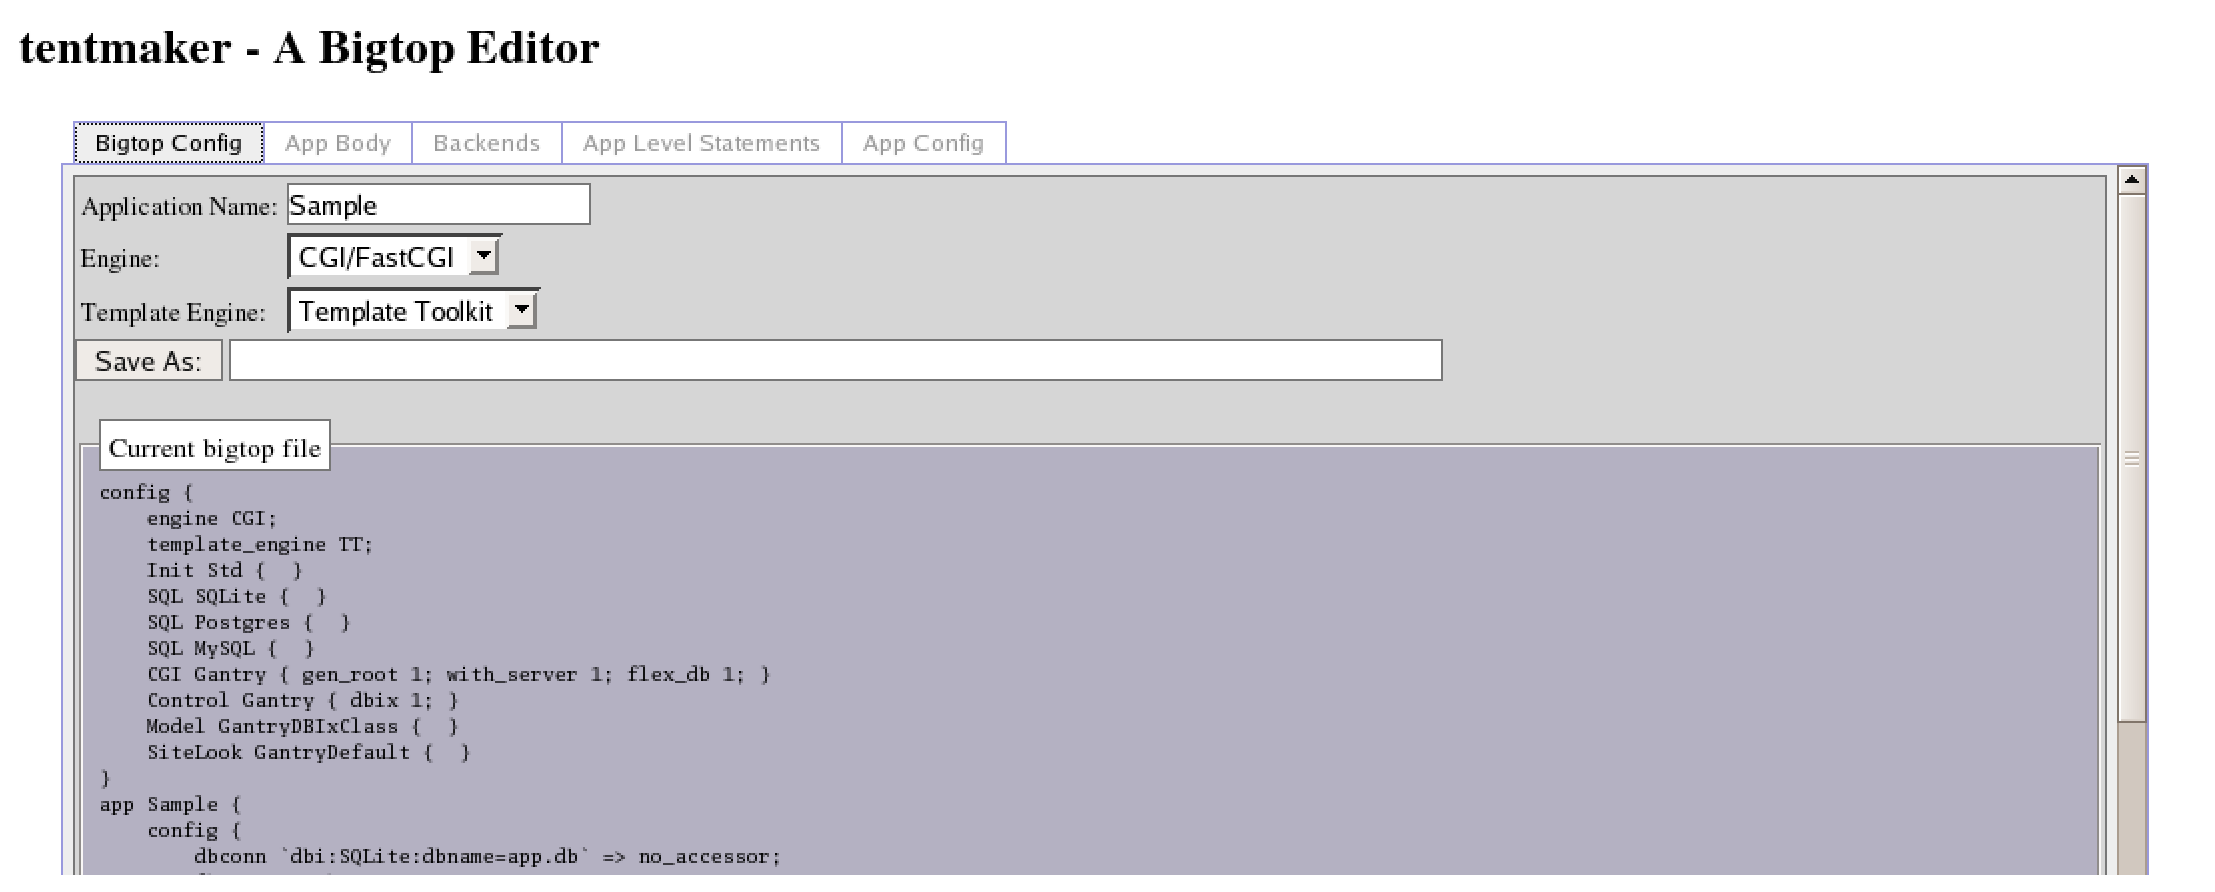
\includegraphics[width=6in]{tentopening}
\caption{The opening appearance of tentmaker.}
\label{fig:tentopening}
\end{figure}

There are five tabs which let you describe your app:

\begin{tabular}{l|l}
Tab Label & Allows you to specify... \\
\hline
Bigtop Config &
    the name of the app and a choice of engines which will serve it \\

App Body &
    the meat of your app, i.e. your tables and controllers \\

Backends &
    the list of all things bigtop should make for you, use check boxes \\
 &  to choose what you want it to do, and input boxes to configure \\
 &  each backend's output \\

App Level Statements &
    author names, their email addresses, project license, etc., all of \\
 &  these have nice defaults \\

App Config &
    a single input table for configuration of your app \\
\end{tabular}

Here we will walk through them in detail.

\subsection*{Bigtop Config}

Let's start at the bottom and move up it.  At the bottom is a dump of the
current bigtop output.  This is mostly for debugging purposes, but look
it over periodically as you have interest.  It is sometimes helpful
when tracking problems.

Immediately above the dump is a `Save As:' button and a file name
box.  When you've made constructive changes, double check the file name and
press the button.  A message will appear, immediately below the button,
telling you how that went.

The top of the tab is more interesting.  Here you can change the name of the
app (which is much easier before initial generation).  You can also choose
a server engine and a template engine.  It is slightly eaiser to start with
the CGI engine and Gantry's stand alone server.  In Chapter \ref{chap:deploy},
we saw how to move to \verb+mod_perl+.

In our shop we like Template Toolkit well enough that we have not added
support to Gantry for any other templating system.  The other alternative
is Default, which turns off templating.  Even with tempating off, you
can still get HTML generation help from Gantry.  The case study in
Chapter \ref{chap:contactus} does this.  You can even use the Template
Toolkit engine manually, when you need to construct special output like
AJAX responses, see Chapter \ref{chap:jobadsapp} for an example.

That is really all there is to say about the first tab.

\subsection*{App Body}

We already had a quick tour through the app body in some prior chapters.
Here we will walk more slowly.

The app body is made up of one or more blocks and statements.  All statements
are managed on the `App Level Statements' tab.  Each block has a type,
most have names.  In the bigtop source file, config is one of the app body
blocks.  It has its own tab (see the last subsection below).  All of the
other types are managed through this tab.

Here are the blocks you can create:

\begin{tabular}{l|l}
Type & Description \\
\hline
Table      & makes an SQL table and corresponding controller              \\
Controller & makes a perl module                                          \\
Literal    & puts literal text into one or more output files              \\
Join Table & indicates two tables which share a many-to-many relationship \\
Sequence   & (rarely used) makes an SQL sequence and corresponding        \\
           & table and controller (useful for Postgres only)              \\
\end{tabular}

Let's look at what you can edit about each of these.

\subsubsection*{Table}

When you open a table for editing, you see something like Figure
\ref{fig:tableedit}.

\begin{figure}
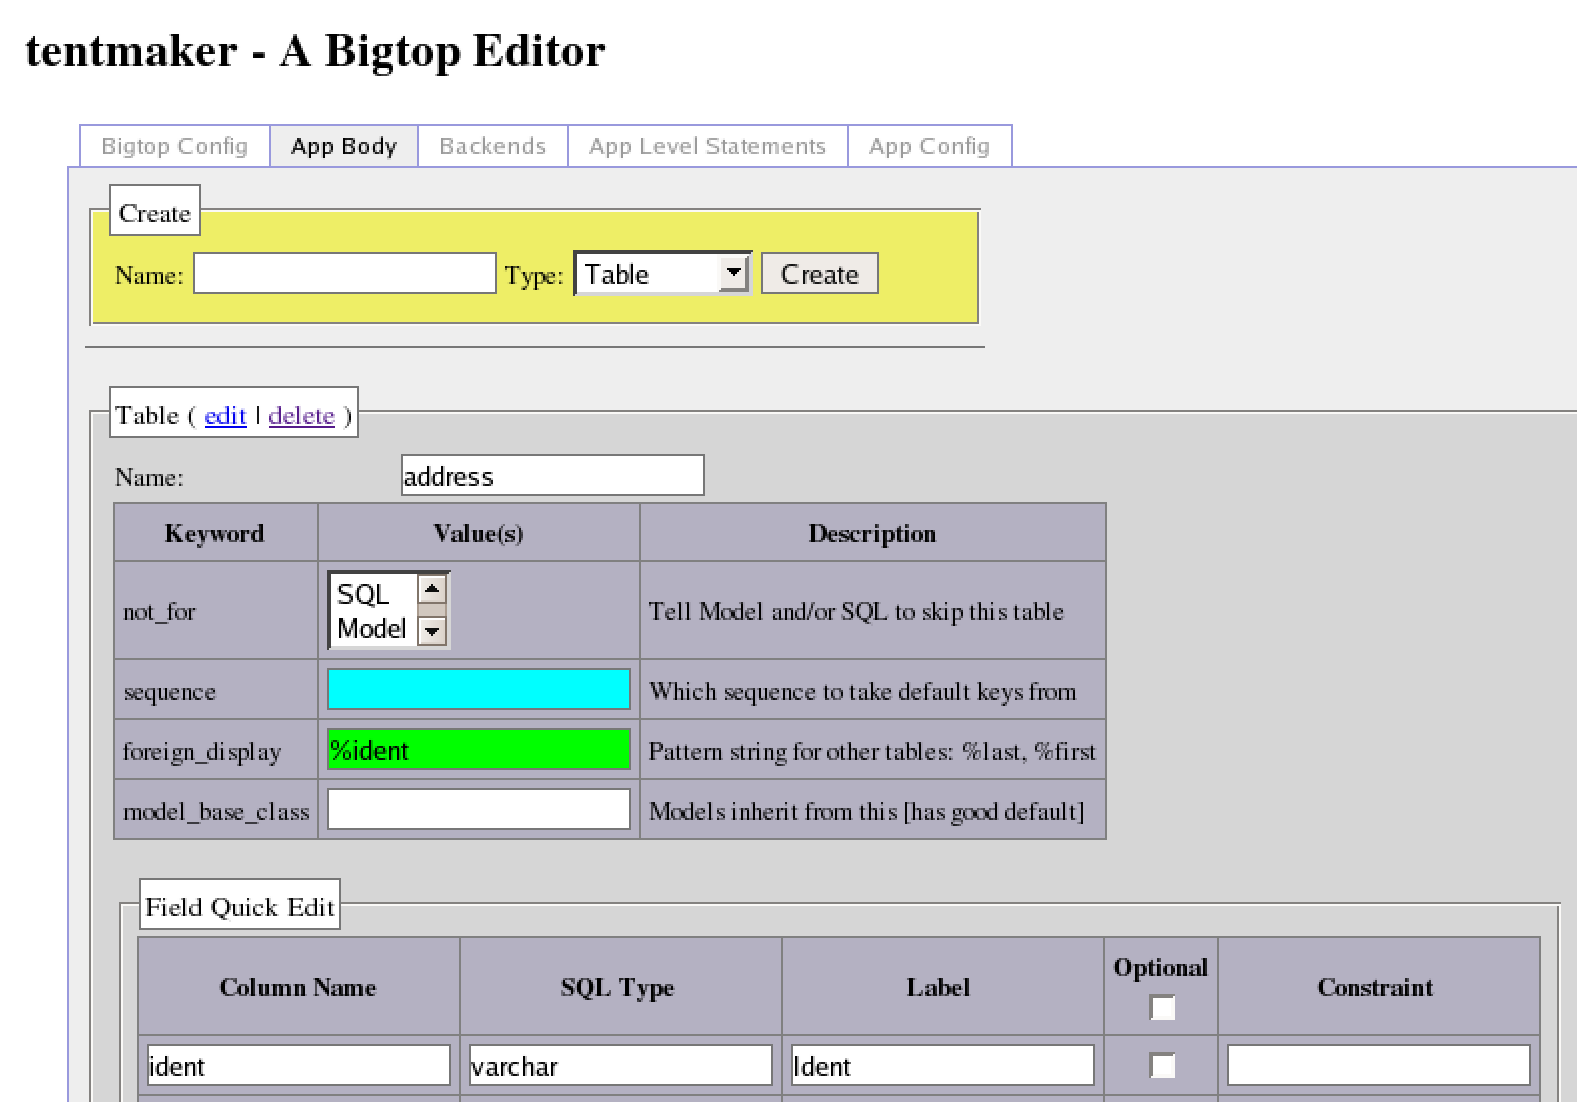
\includegraphics[width=6in]{tableedit}
\caption{Editing a table in tentmaker.}
\label{fig:tableedit}
\end{figure}

From this we see four statements which affect a whole table.  If the table
might offend one of the backends, you can highlight \verb+not_for+ for
that backend.

If you did use a sequence (which we are moving away from) enter its name
in the \verb+sequence+ box.  If you had tentmaker build the sequence for you, it
should have filled that in.

You should probably have a \verb+foreign_display+.  It governs the sort order
of the table when users see all the rows.  It also the summary users will
see when other tables refer to this one via a foreign key.  For example,
if users will select one row from this table as the foreign key value of
another table, this is what they will see in the pull down menu.

The format for \verb+foreign_display+ is simple.  If an ident follows a
percent sign immediately (without whitespace in the middle), it must
be a column name which will be interpolated in at that point.  Everything
else, including trailing percents, is literal.  A common example is
\verb+%last_name, %first_name+, but you can do whatever you like.  Keep in
mind that brevity will probably be appreciated by your users.

Most models should inherit from the default base class, which depends on
the Model backend you choose on the `Backends' tab.  If all of your models
need to inherit from a different base, change it once on the `Backends' tab.
If just this table needs a different base, enter the fully qualified
parent module name here.

Though tables have statements, their main purpose in life is to house
fields.  Fields become columns in the database table and (usually) entry
widgets on the screen.

When you open a field for editing, you see something like Figure
\ref{fig:fieldedit}.

\begin{figure}
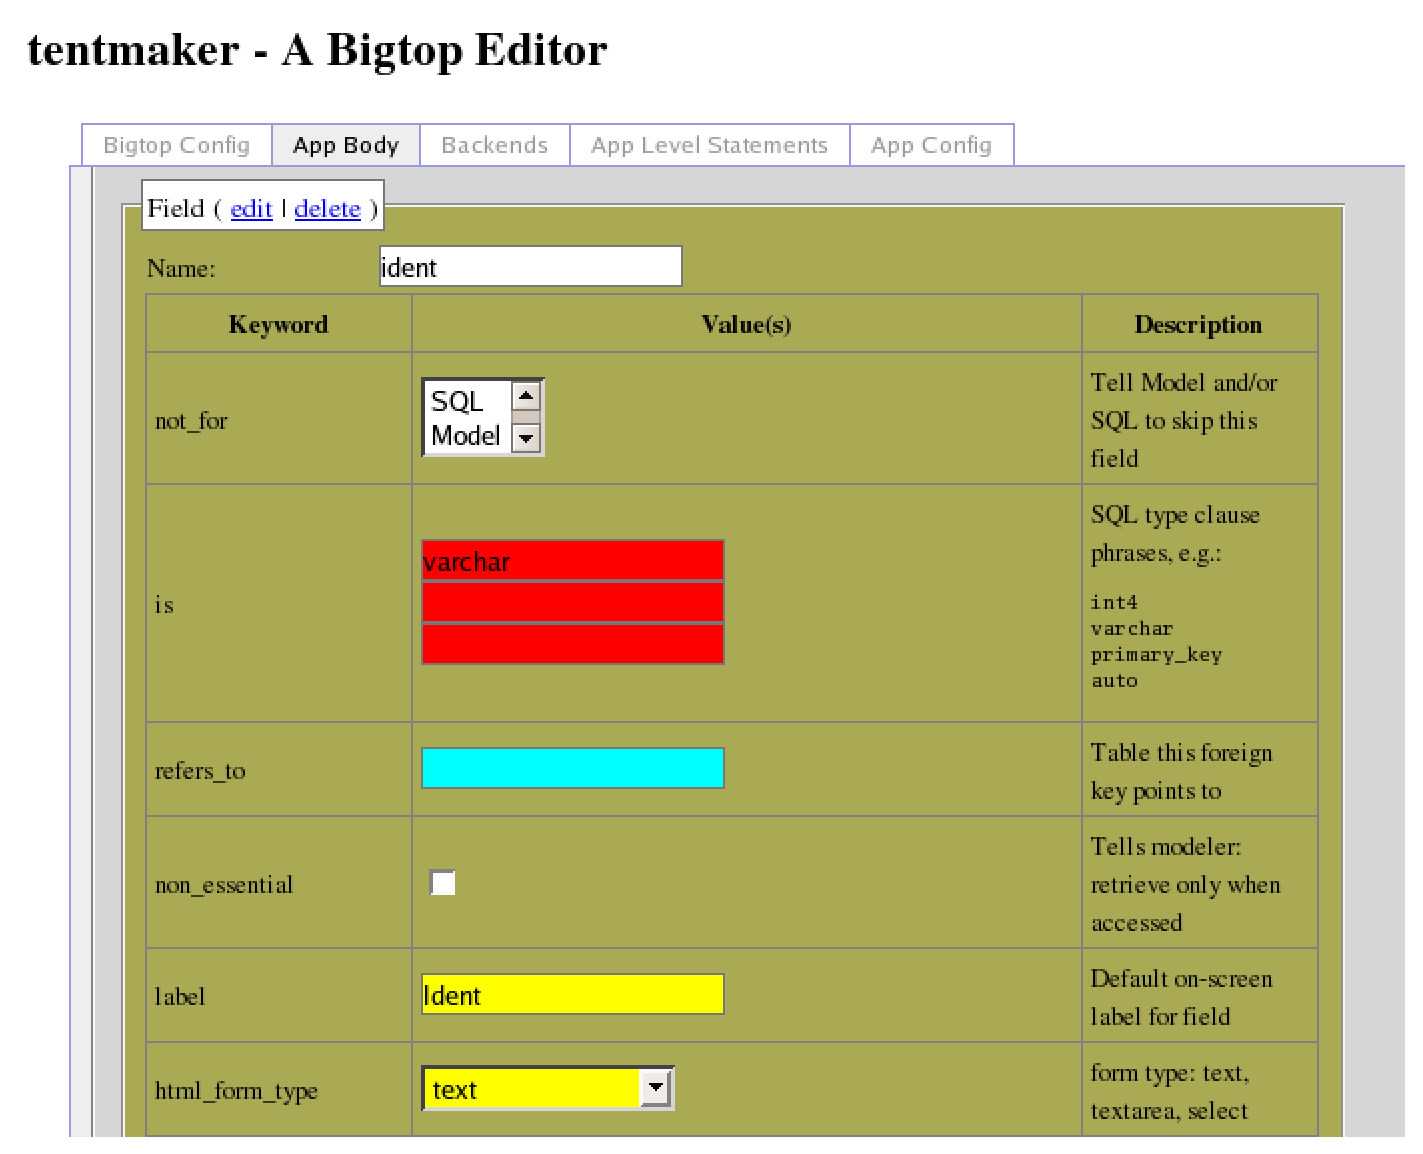
\includegraphics[width=6in]{fieldedit}
\caption{Editing a field in tentmaker (same as Figure \ref{fig:fieldedit1}).}
\label{fig:fieldedit}
\end{figure}

There are many statements that affect fields.  The \verb+not_for+ statement
works for fields just as it does for tables.  This is useful if you have
a column called id which is not the primary key, a situation that confuses
some ORMs.

The \verb+is+ statement accepts SQL phrases for the column defintion.
The most common value is \verb+varchar+, which the backends will translate
to a good string type, if your database doesn't understand it.

You can put as many items in the \verb+is+ statement as you like, one per
box.  There are two highly special items: \verb+primary_key+ and \verb+auto+.
Use \verb+primary_key+ to specify your primary key.  Currently Bigtop and
Gantry don't have much support for multi-column primary keys.  So we
usally stick with the id generated on table creation.

Use \verb+auto+ to indicate that the primary key should be incremented
by the database.  Exactly how that happens is up to the SQL backend
for your database.

The \verb+refers_to+ statement indicates that this column is a foriegn
key pointing to another table.  The other table's name is the value.

Some ORMs use lazy column fetching.  If yours does and the current column
should be fetched lazily (only when an accessor for it is called), check
the \verb+non_essential+ box.

The \verb+label+ is what the user sees whenever the field is on screen.

All of these directly become attributes of the html form elements:
\verb+html_form_type+, \verb+html_form_cols+, \verb+html_form_rows+,
\verb+html_form_display_size+.  The last one becomes the size attribute
of a text input area, since Template Toolkit has a virtual method called
size.

By default, all fields on a form are required.  If you want a field
to be optional, check \verb+html_form_optional+.

The \verb+html_form_constraint+ is used directly by Data::FormValidator,
see its docs for details of what you can put in it.  The short answer
is a regex or a method which returns one.

Any \verb+html_form_default_value+ will be used by the form template
when there is nothing better avaiable.  It must be a literal string or number.

If you want to use a popup date calendar, for a field of type date,
enter a \verb+date_select_text+.

The only statement left is \verb+html_form_options+.  Use this to
enter the options for fields whose \verb+html_form_type+ is select,
unless the field is a foreign key.  Foreign key fields have good
generated selections.

The `Label' of an \verb+html_form_options+ entry is what the user
sees.  The `Database Value' is what goes into the database.  As you
enter options, more boxes appear underneath.  Options appear in the
order the appear in tentmaker.  If you make an error in ordering,
it is usually easier to fix it in a text editor.

\subsubsection*{Controller}

Each controller represents a pair of code modules: a stub module and a GEN
module.  Once written, stubs are never overwritten.  The only ways to get
bigtop to regenerate a stub module are to rename or delete it.

When you edit a controller, you'll something like Figure
\ref{fig:controledit}.

\begin{figure}
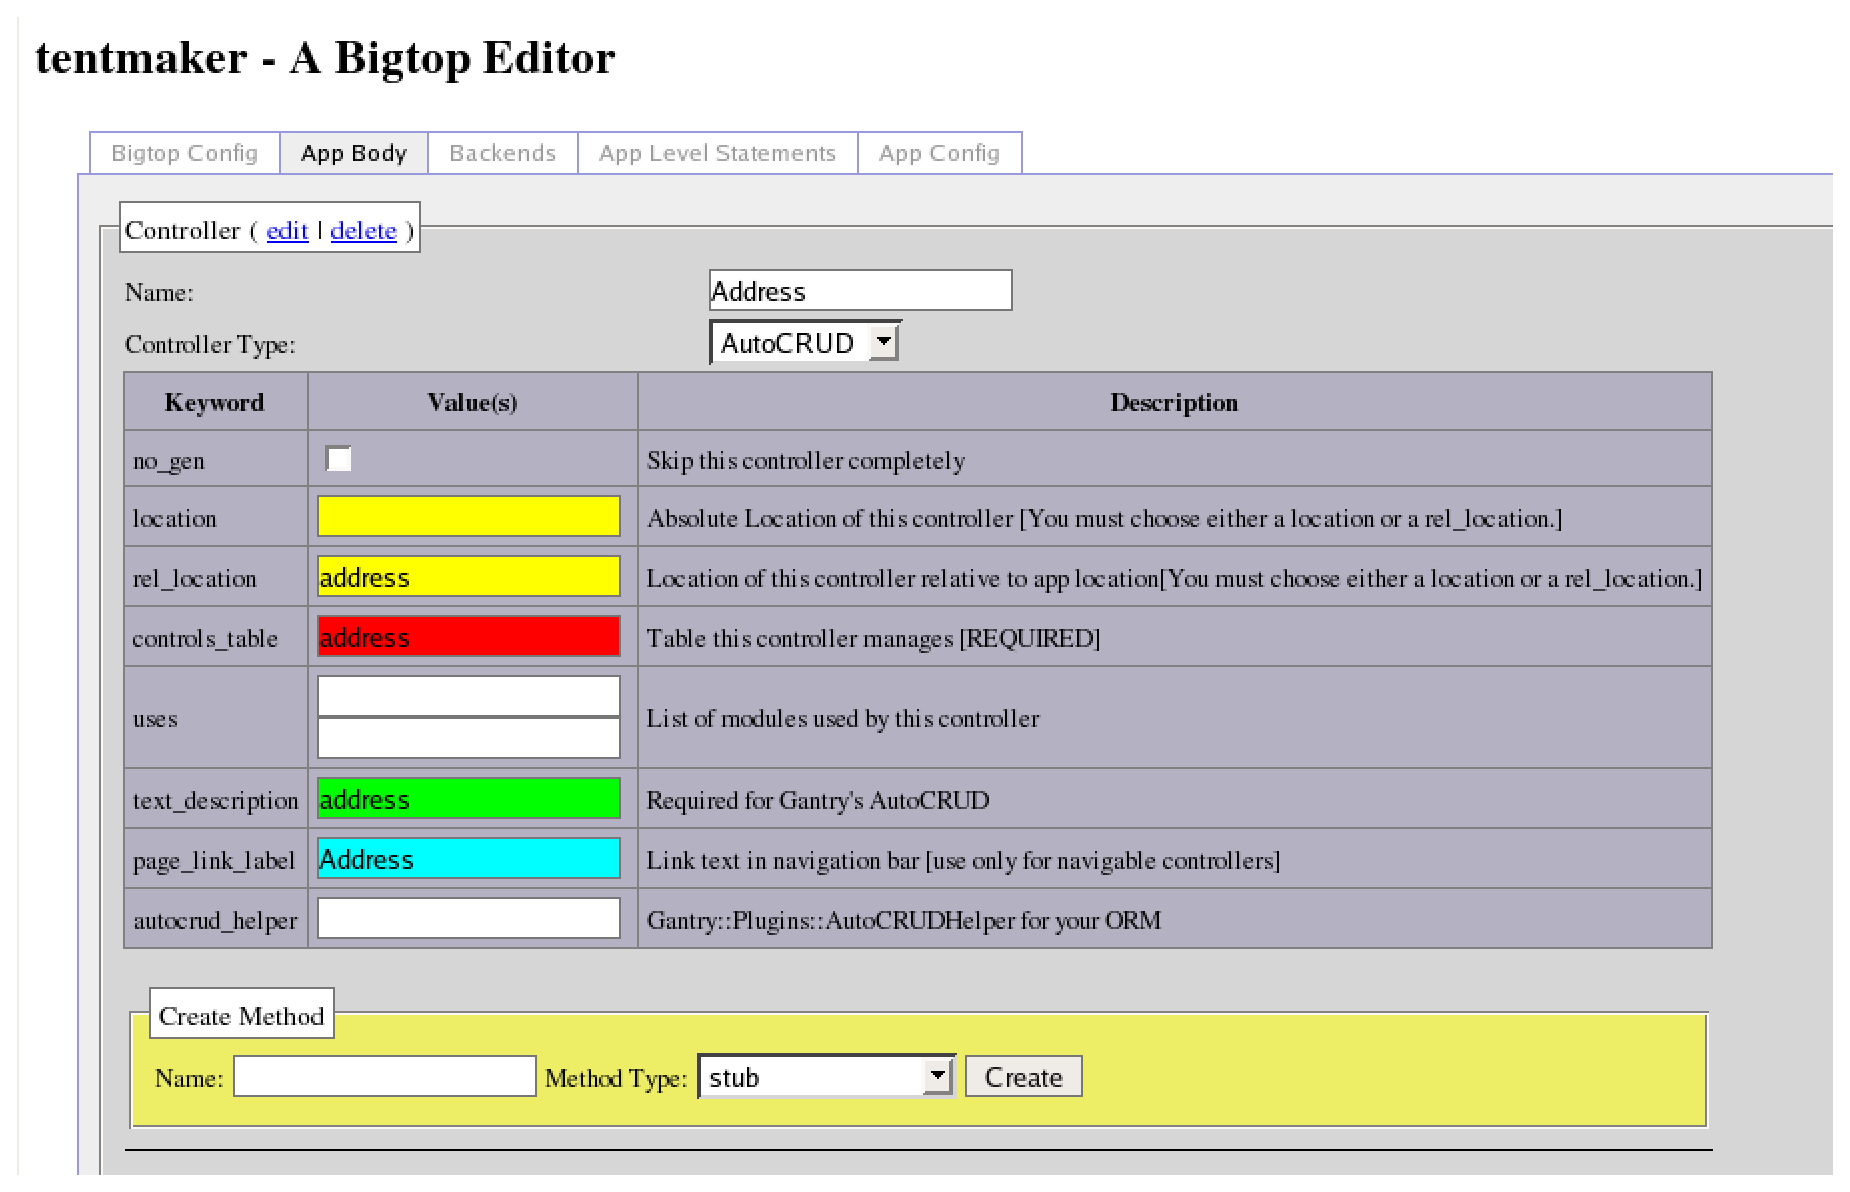
\includegraphics[width=6in]{controledit}
\caption{Editing a controller in tentmaker.}
\label{fig:controledit}
\end{figure}

If you want to skip just one controller, check the \verb+no_gen+ for it.

You must supply either a \verb+location+ or \verb+rel_location+.
\verb+location+ is absolute, \verb+rel_location+ is relative to the
base location for the app.

Most controllers control a single table, enter its name in the
\verb+controls_table+ (if it isn't already there).

If your controller needs external modules, put them in \verb+uses+ boxes.
But, keep in mind that these are most useful in the stubs.  So, using
these won't work after the controller is generated.

The \verb+text_description+ fills in the blank in several sentences for
AutoCRUD.

If you want this controller to appear in site navigation links, give
it a \verb+page_link_label+.  The user will click this label to advance
to this controller's page.

If you have your own ORM scheme, but it doesn't have a backend, specify
an \verb+autocrud_helper+.  It must be a module which responds to the
expected API.  See Chapter \ref{chap:autocrud} for advice.

In addition to the statements in a controller block, there are methods.
When you open a method for editing you see something like Figure
\ref{fig:methodedit}.

\begin{figure}
\includegraphics[width=6in]{methodedit}
\caption{Editing a method in tentmaker.}
\label{fig:methodedit}
\end{figure}

Notice that there is a applies to column in the table.  It tells you which
types of methods can use the statement.

There are three types of methods: stubs, main listings, and forms.  A
stub is just that.  A typical one looks like this:

\begin{verbatim}
#-----------------------------------------------------------------
# $self->stub_name(  )
#-----------------------------------------------------------------
sub stub_name {
    my ( $self ) = @_;
}
\end{verbatim}

You can check \verb+no_gen+ for any method type, causing the backend
to skip it.  You can also supply \verb+extra_args+ for any method these
are added to the end of the argument list at the top of the method
(and in the docs).  Put one argument in each box, remember to include
the sigil.  Further, realize that if the argument is an array, it must
go at the end.

Stub methods are not that much use.  Keep in mind that they only go in
stub modules, so they won't be added once the controller is initially
generated.  The other types are more useful.

The main listing output typically shows all the rows from a simple table
as shown in Figure \ref{fig:main_listingout}.

\begin{figure}
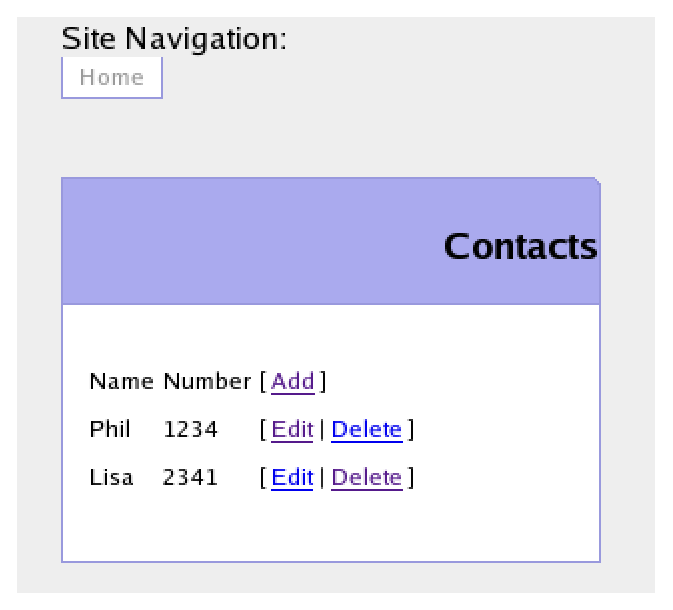
\includegraphics[width=6in]{main_listingout}
\caption{Editing a method in tentmaker.}
\label{fig:main_listingout}
\end{figure}

The \verb+cols+ list names each column of the main listing table.  By
default, these columns are labeled with their field's label.  If you want
to change the label just for the main listing, enter your alternate
labels in the \verb+col_labels+ boxes.  Of course, these must be in the
same order as the \verb+cols+.  Less obviously, skipped boxes are ignored,
not counted.  If you don't supply the same number of labels as their
are columns, the extras will revert to default naming.

At the far right of the main listing output in Figure
\ref{fig:main_listingout}, you see a link labeled `Add.'  That is a
\verb+header_option+.  You can have as many of these as you like.
Normally, they will be handled by a method in the same controller as
the main listing.  The name of the method will be the same as the
label, but in lower case.  If you want a different method to handle
the action, put its location in the `Location,' column.  Even if
some of the `Labels' have alternate `Locations,' you don't have to
specify locations unless the default won't work.

The \verb+row_options+ are similar to \verb+header_options+, but they
apply to each row in the listing.  The most common of these are `Edit'
and `Delete.'  The rules for their locations are the same as for `Add.'
If you construct your own locations, you will want to remember to include
\verb+$id+ at the end of the URL or a query string with that id in it.
Otherwise, the row will be unknown at edit time.

The \verb+title+ is the browser window title.  The \verb+html_template+
defaults to \verb+results.tt+, change it if you like.

All of the remaing statements apply to form methods.  Note that form methods
come in two kinds.  One is for use with AutoCRUD, the other for CRUD.
Their statements are exactly the same.  They only differ in how they
capture their arguments.

The key feature of a form is that it displays a set of entry fields for
columns in the underlying database table.  The first step in setting
one up is to pick the fields.  There are two ways to do that.  Either
enter the fields you want, each one in its own \verb+fields+ input box;
or enter the fields you don't want, each one in its own \verb+all_fields_but+
input box.  I usually do that latter.  That makes it less work when
new fields are added to the table, because in the normal case I want to
enable users to update the new field.

Form methods build hashes which are passed to templates.  Some templates --
including the default form.tt supplied by Gantry -- allow additional
hash keys tentmaker doesn't know about.  The \verb+extra_keys+ take care
of this case. recall that Section \ref{sec:asciiart} has an example involving
a popup calendar.

If your form needs a name (e.g. for CSS use or a popup calendar), enter
it in the \verb+form_name+ input box.

Those are all the statements that apply to methods.  With them, we have
finished talking about controller edits.

\subsubsection*{Literal}

Literals are taken literally.  Each one is understood by at least on backend
or backend family.  They take text directly from your bigtop source file
and dump it into their output.

There are several literal types, this table shows them along with an
explanation of where their output goes.

\begin{tabular}{l|l}
Literal Type & Output Destination \\
\hline
SQL       & docs/schema.*, for all of your SQL backends \\
Location  & the base module location in httpd.conf made by HttpdConf Gantry \\
HttpdConf & between locations in httpd.conf made by HttpdConf Gantry \\
PerlTop   & immediately below the shebang line in <Perl> block of httpd.conf \\
PerlBlock & inside the <Perl> block of httpd.conf \\
Conf      & at the top level of Config::General conf file \\
\end{tabular}

Note that all of the literal types are always legal, but they will be ignored
unless a loaded backend understands them.

When I said that literals are taken literally, I left out one obscure
but pleasant exception.  If your literal does not end with whitespace,
one new line will be added to it in the output.  Otherwise, they are
taken as written.  But, note that how they look in the input box on
the `App Body' tab of tentmaker may be decieving, since some characters
are not visible there (like trailing spaces).  To be sure of what is
in your literal, look at the `Current bigtop file' dump on the `Bigtop
Config' tab.  You could also look at the bigtop file with a text editor.

\subsubsection*{Join Table}

A join table is needed whenever two tables share a many-to-many
relationship.  This table will alwyas have three columns: its own id
and the foreign key ids of the many-to-many tables.  Editing a join
table looks like Figure \ref{fig:joiner}.

\begin{figure}
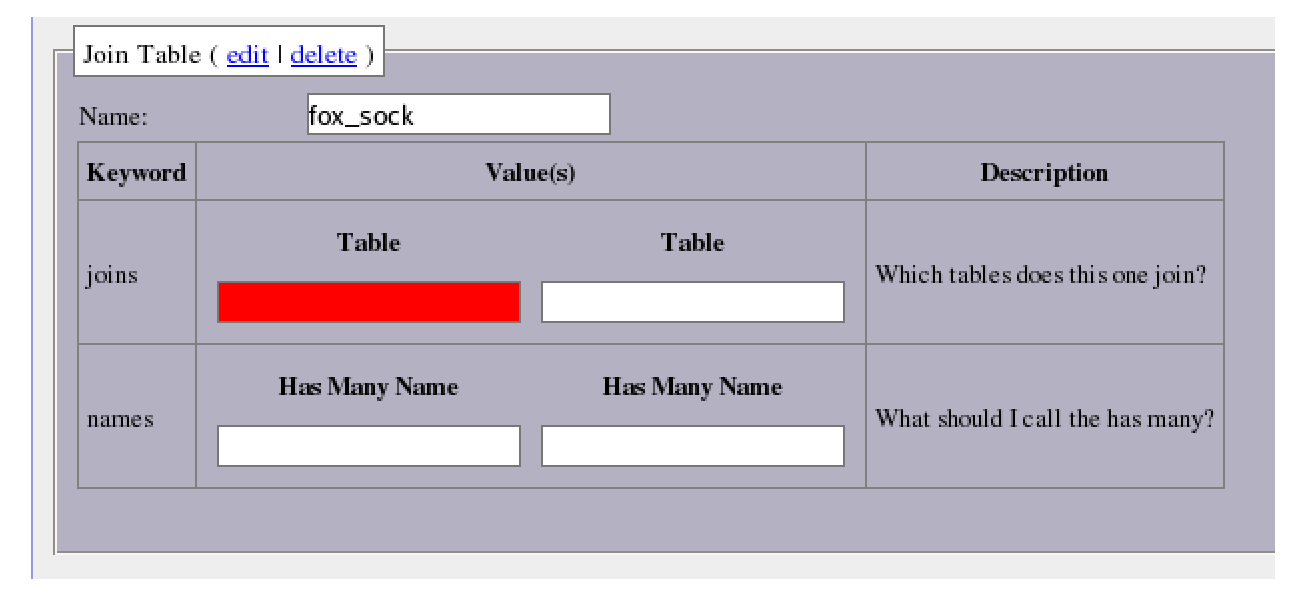
\includegraphics[width=6in]{joiner}
\caption{Editing a join table in tentmaker.}
\label{fig:joiner}
\end{figure}

When using a join table, you must specify the names of the tables it
\verb+joins+ (even if a bug in the CSS doesn't make both boxes red).

For the models to have a many-to-many relationship, you need to use
the Model GantryDBIxClass backend.  It is the only one that understands
them.

Each side of a many-to-many relationship needs a name.  Normally, the
name is the table name with an extra `s' added at the end.  But,
you can control the \verb+names+.  If you pick one, you must pick the
other, even if your choice would be the default.  In Figure \ref{fig:joiner},
the \verb+names+ should probably be `foxes' and `socks.'

A join table is made for you when you use \verb+<->+ in ASCII art for
bigtop or tentmaker.  See Section \ref{sec:asciiart}, or the first section
of this chapter, for how to do that.

\subsubsection*{Sequence}

If you like to use Postgres sequences to auto-increment your primary key,
feel free to create a sequence for each table.  Do this at the outset,
because sequences must be defined before the tables which use them and
because creating a sequence in tentmaker makes a corresponding table
and controller.  Name the sequence with a trailing \verb+_seq+.  Then
the names of the table and controller will make more sense.

Using sequences is not a problem, even if your database does not understand
them.  The backends whose databases don't support them correctly adjust to
a sequence if it is present (mostly by ignoring it).

\subsection*{Backends}

Bigtop can make lots of different things.  The Backends tab controls what
it makes for you.  The basic idea on this tab is simple.  Check the box
for each backend you want working for you.  Once the box is checked, fill
in any values you need for that backend.  See Chapter \ref{chap:backends}
for a list of all available backends and what their configurable values.
When you click the `Backends' tab, you see something like Figure
\ref{fig:backends}.

\begin{figure}
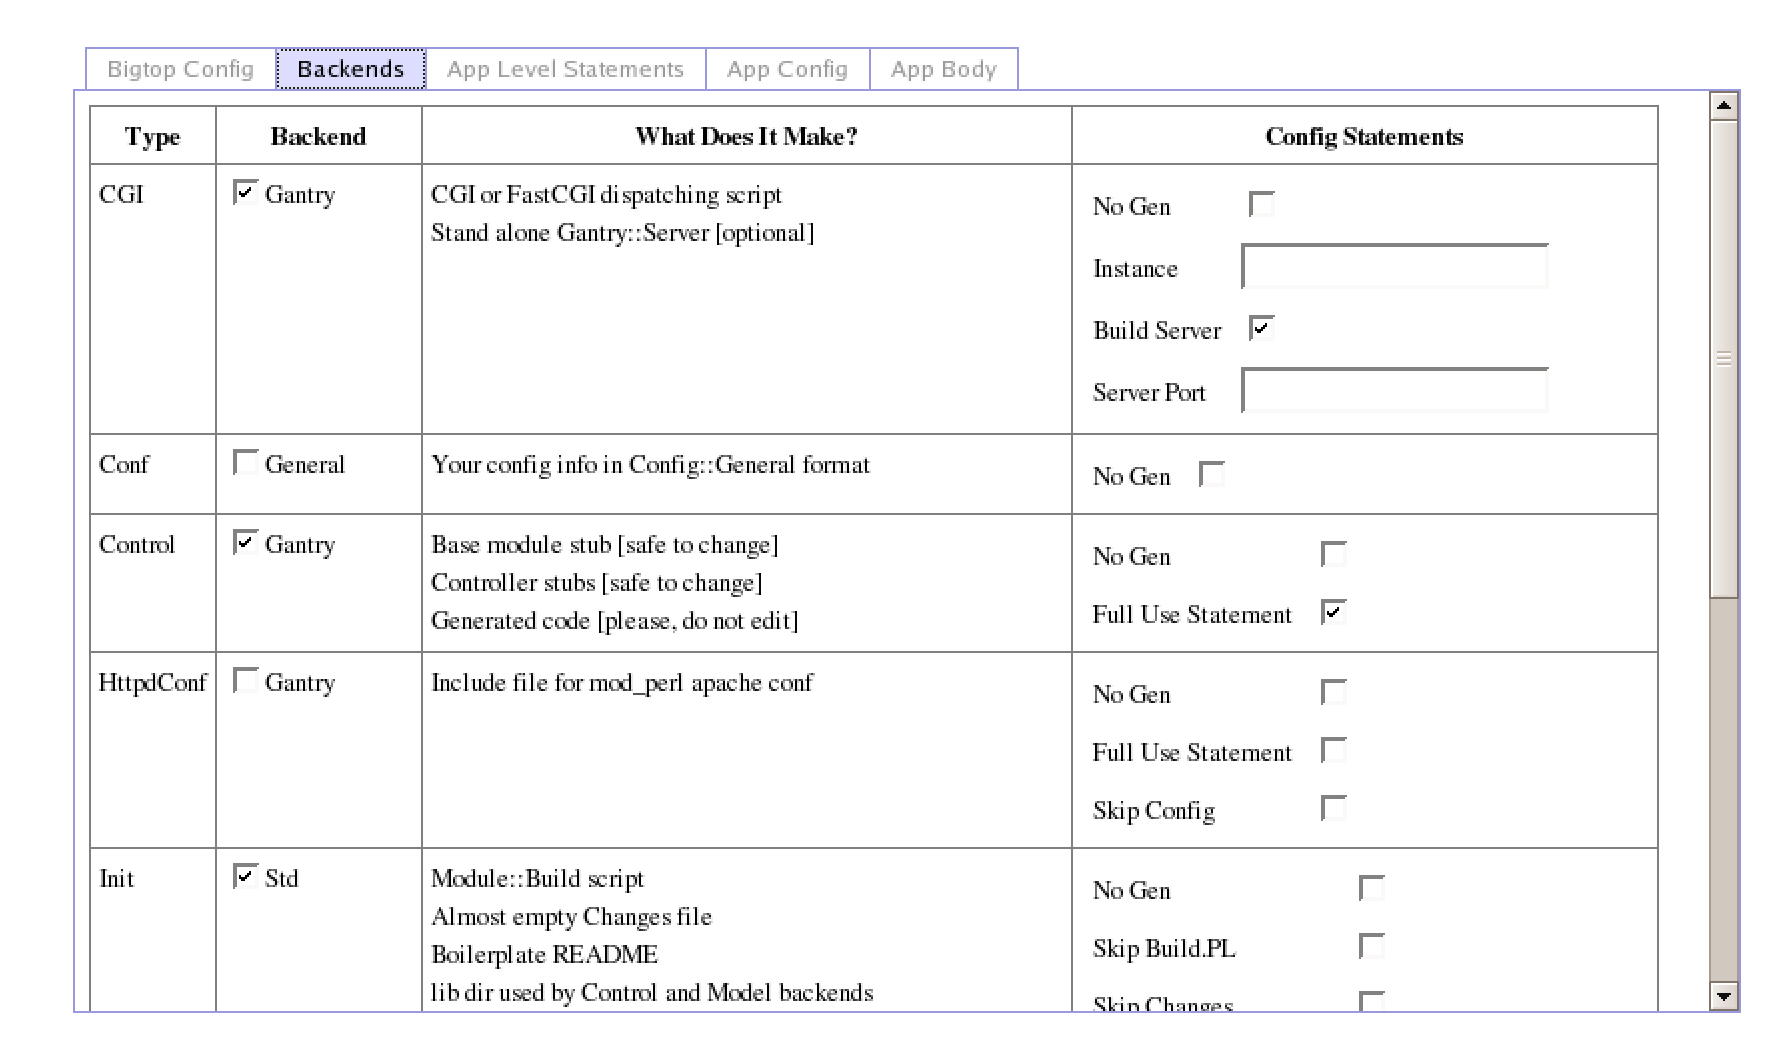
\includegraphics[width=6in]{backends}
\caption{The top of the backends tabbed pane, showing typically available
backends.}
\label{fig:backends}
\end{figure}

I've refrained from including addtional screen shots featuring the othter
backends.  The modules which support tentmaker know how to find all the
backends on your system, so any new ones will show up when you run tentmaker
(see Part IV for how to make your own backends).

Since Chapter \ref{chap:backends} covers them, we'll move along now.

\subsection*{App Level Statements}

App level statements describe the application and its base Perl module.
You must update all of these statements before generation, except `Base
Location.'  Once the base module for the app -- or any other stub module -- is
generated, it is never regenerated.  Bigtop will cowardly refuse to
regenerate stubs.  There is no way to force it to rewrite a stub file short
of deleting or renaming it.

When you edit a default bigtop file, all the app level statements are
blank, so the `App Level Statements' table looks like Figure
\ref{fig:appstat}.

\begin{figure}
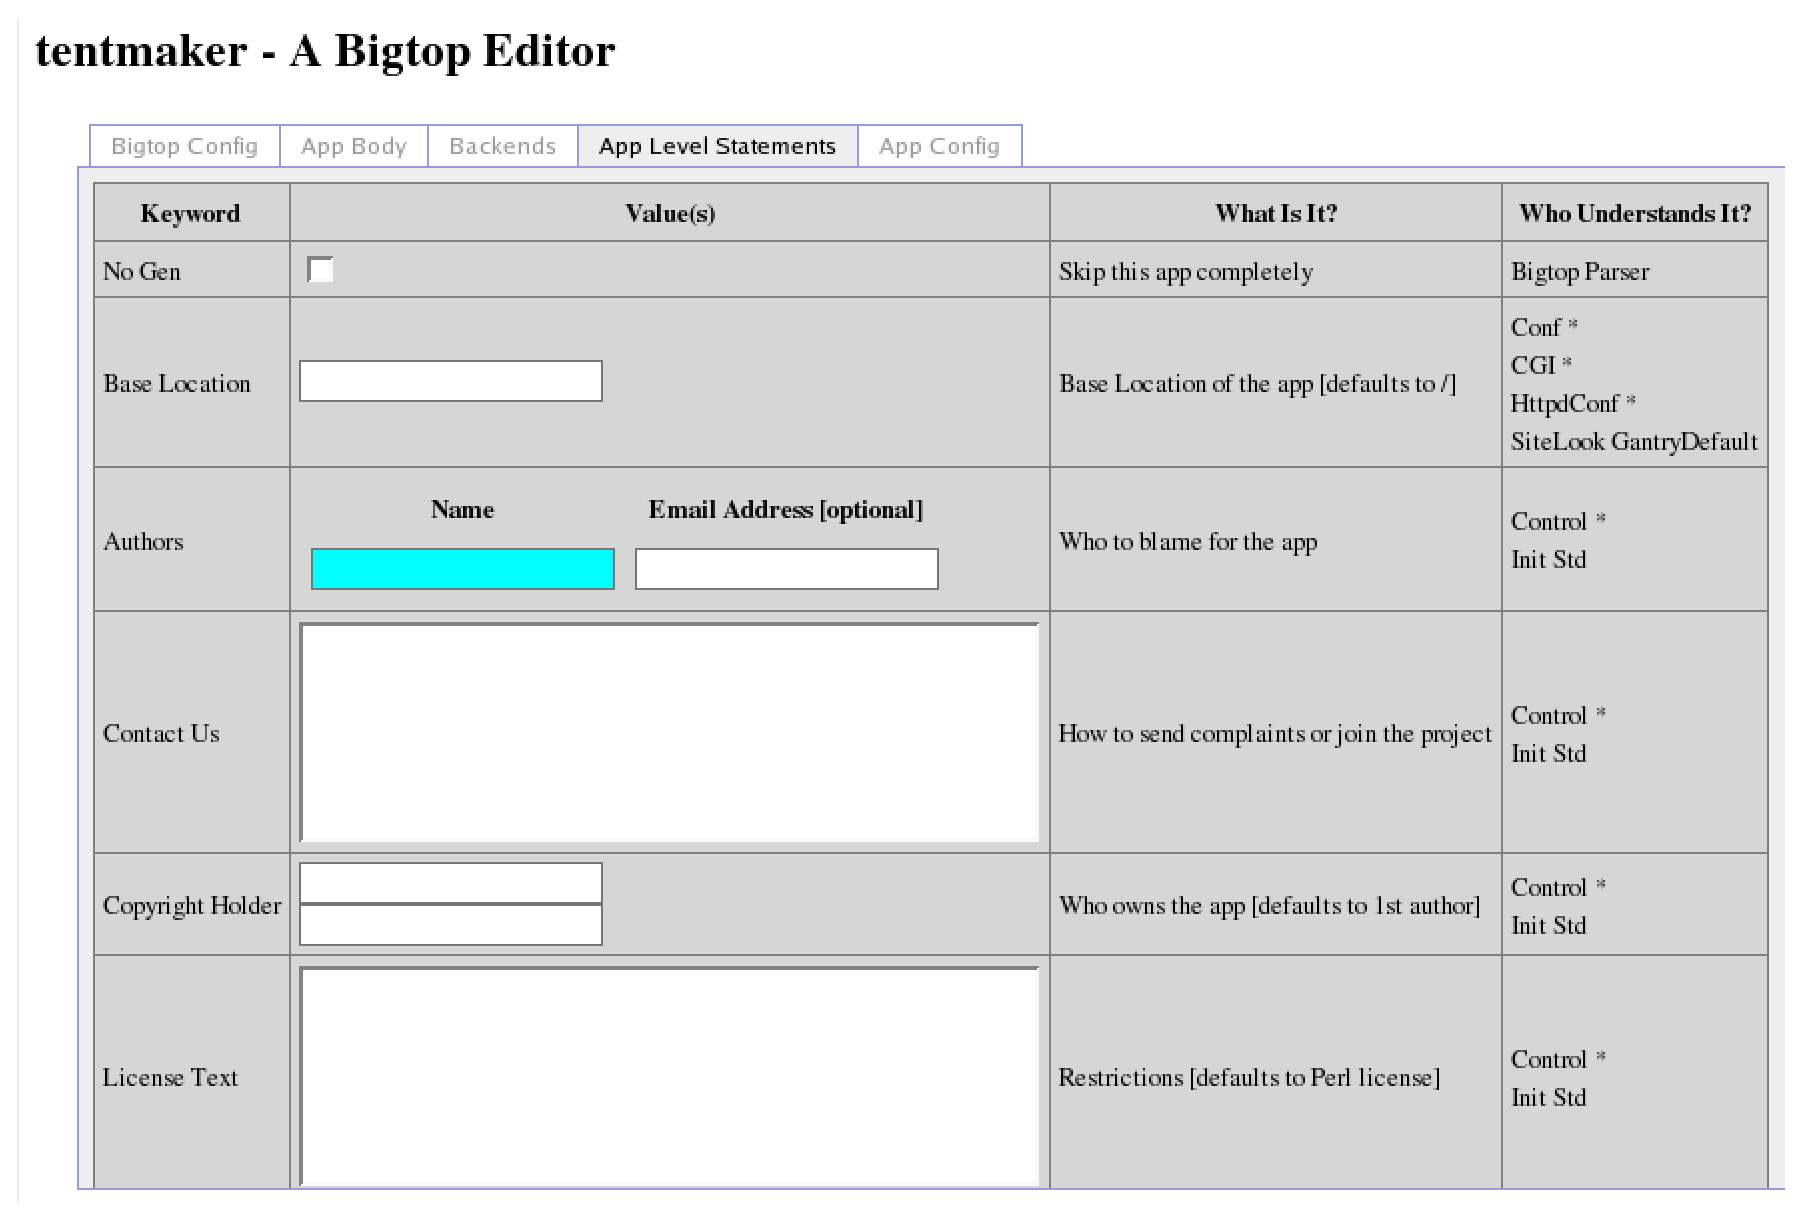
\includegraphics[width=6in]{appstat}
\caption{Editing app level statements in tentmaker.}
\label{fig:appstat}
\end{figure}

All of the things on this tab are optional and have fine defaults.

Truly paranoid people might want to check the `No Gen' box.  Doing
so make the bigtop script skip all generation.

The `Base Location' is the beginning of the URL for all pages in the app.
It is safe to leave it blank.  Then all pages will be at the document
root of the server.  You cannot use a non-trivial `Base Location' with
a stand alone server (like app.server), because it doesn't have a document
root notion.  When you do set a `Base Location,' you need to add an
\verb+app_rootp+ config variable with the same value on the `App Config'
pane (see the next subsection).

If you never enter \verb+authors+, the author name and email will be generated
just like h2xs generates them.  If you do enter `Authors,' you may choose
to supply email addresses.  This is why the name input boxes are colored but
the email input boxes are white.

To add a blurb about joining or contacting your project developers to
various generated docs, enter something for `Contact Us.'

If the first author is not the copyright owner, enter the proper
`Copyright Holder.'

By default, the license text is the same as what h2xs generated for
the Perl 5.8.6 distribution.  If you want something different, enter it
in `License Text.'

Out of view in Figure \ref{fig:appstat} is the `Modules Used' list.  These
will be included in \verb+use+ statements at the top of the base module.
But, keep in mind that the base module will only be written once, so
changes here won't affect one already on your disk.

\subsection*{App Config}

Finally, we come to that last tab.

Most apps have some configuration parameters which should be kept out of
the code, enabling administrators to update them on production machines without
disturbing our beautiful modules.  The `App Config' tab lets you
specify these.  If you started tentmaker without command line data,
there will be three config params already defined, as shown in Figure
\ref{fig:appconfig}.

\begin{figure}
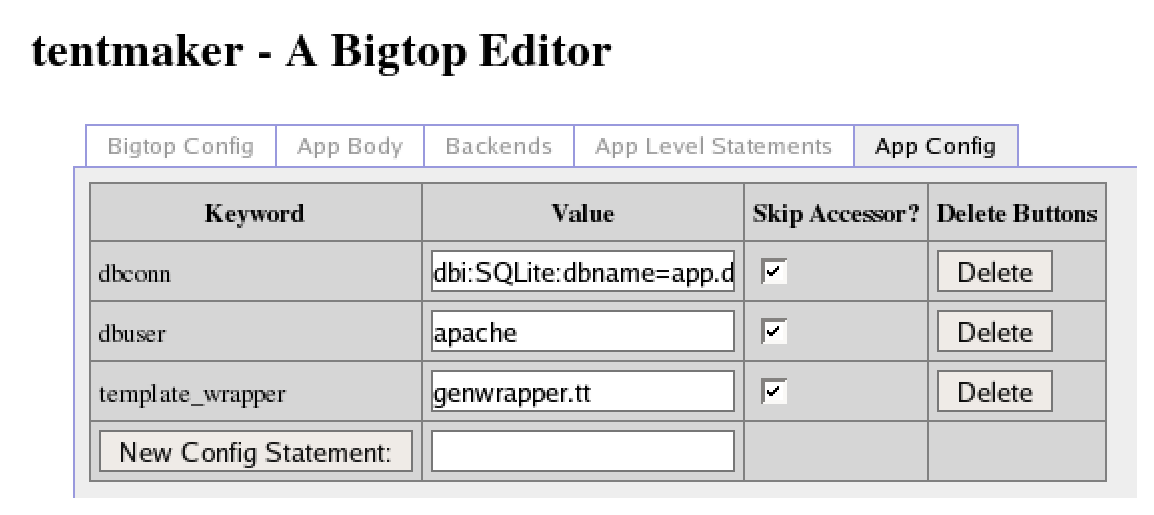
\includegraphics[width=6in]{appconfig}
\caption{Application configuration table.}
\label{fig:appconfig}
\end{figure}

Here you see the DBI connection string.  By default this will use SQLite
as the DBD and call the database app.db.  In earlier examples, we saw
that the stand alone app.server allows users to change this information
at the command line.  In fact, app.server pays no attention to the database
config parameters.  In CGI/FastCGI and \verb+mod_perl+, the information
from the dbconn, dbuser, and (optional) dbpass variables here completely
governs.

By default \verb+template_wrapper+ is set to \verb+genwrapper.tt+.  You
can change that at will to your own wrapper.  The SiteLook GantryDefault
backend makes \verb+genwrapper.tt+.  If you've rolled your own, you don't
need that backend, but you do need to set the name of your wrapper here.

If there are any other config parameters your app needs, feel free to
add them.

Now that we know what tentmaker can already do, you are ready to think big.
But, if you prefer typing to clicking, read the next chapter.  It covers
the syntax of the Bigtop language.  Once you know that, you can type Bigtop
files directly.  More likely, you'll use the information to edit Bigtop
files made by tentmaker.

The subsequent chapters explain how to customize Bigtop to build whatever
you need for your apps.  As you build things, they become available
through tentmaker as soon as you install them on your system (or sooner
if you add a use lib to your tentmaker).
